\documentclass[a4paper,10pt]{article}
\usepackage[francais]{babel}
\usepackage[utf8x]{inputenc}
% Title Page
\title{RAPPORT MOIA-SCS\\
            Hive}

\author{\\Amine TALBI - Hugues FAGNINOU}
\usepackage[final]{pdfpages}
\usepackage{graphicx}

\begin{document}
\maketitle
\newpage
\tableofcontents
\newpage
\section{Introduction} 
Le projet de MOIA de cette année consiste à établir les règles de jeu du hive en
modélisant le plateau et 
les pièces du jeu en prolog. Les prédicats de déplacement doivent tenir compte
des contraintes du jeu (
la reine est posée au 4 ème tour au maximum, aucun déplacement ne peut avoir
lieu tant qu'on a pas posé notre
reine,...).
\section{Modélisation du Hive en prolog}
La modélisation est la partie la plus importante du codage du jeu. En effet après tout déplacement le plateau doit être 
mis à jour. La qualité du modèle se mesure à la facilité à actualiser notre
liste après n'importe quel coup.
On a opté pour une modélisation par coordonnées absolues. La ruche ressemble à
une grille ou chaque case est
un emplacement potentiel pour chaque pièce. En outre une autre information s'ajoute à notre modèle pour décrire la hauteur
de la pièce (niveau d'empilement).
Le plateau de jeu va ressembler à :                                            
\begin{verbatim}[[identifiant_de_la_Pièce,X,Y,hauteur_de_la_pièce],.......]
\end{verbatim}
La première pièce posé sur le plateau de jeu aura comme coordonnées (0,0,0) est
puis les coups suivant s'ajoutent 
de façon à garder la ruche en un seul bloc.
\begin{center}
 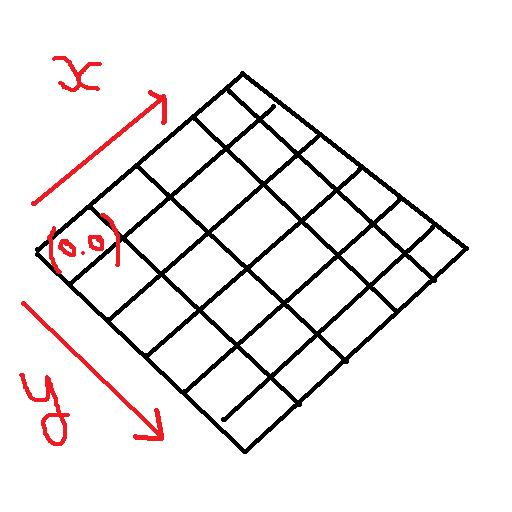
\includegraphics[width=7cm,height=50mm]{testrl.jpg}
\end{center}
%%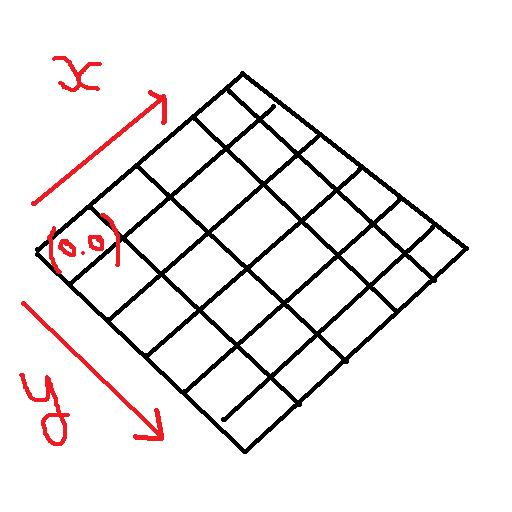
\includegraphics{testrl.jpg}
Ainsi la mise à jour du plateau après chaque coup se fait par l'appel des 
deux prédicats suivant:
\begin{verbatim}retirerPiece(Liste1,PieceJ,Liste2)\end{verbatim}
\begin{verbatim}ajout_debut(X,Liste_Avant_Ajout,Liste_Après_Ajout)\end{verbatim}
\section{Prédicats et enjeux importants}
Le prédicat rucheCasser a été créé pour maintenir la ruche en un seul bloc.
L'idée de ce prédicat est d'utiliser 
deux accumulateurs: Acc1 et Acc2. Acc1 est utilisé pour stocker les pièces
parcourues dont les voisins ne sont pas encore visités.
 Acc2 stocke les pièces de Acc1 avec tous les voisins visités. Quand Acc1
devient vide, on récupère le contenu de Acc2 puis on compare
sa longueur avec le nombre de pièces non empilées. En cas d'égalité, le
prédicat réussie sinon il échoue auquel cas, la ruche a été cassée après le
dernier coup.
\begin{verbatim}
% rucheCasser(Liste, Acc1, Acc2)/3
% Liste   : le plateau de jeu
% Acc1    : La liste des pieces avec les voisins non exploité
% Acc2    : La liste des pieces avec les voisins exploité
% le predicat reussit si le nombre de pièces visitées à partir de
% la premiére liste du plateau est = nombre de pieces dans le plateau de jeu								
rucheCasser([[P,X,Y,Z]|Liste],_,_):-	verifEmpil(Liste,[X,Y,Z]),!.
rucheCasser(Liste,Acc1,Acc2):-  	premier([E,X,Y,Z],Liste),
				    	voisin([X,Y,Z],Liste,[],R),																	  	
					rucheCasser(Liste,R,[[X,Y,0]],Res),
					longueur(Res, R1),
					nbrPieceNoEmpil(Liste,0,R2),		  	
					R1=:=R2.
									  									  								  	
% rucheCasser(Liste, Acc1, Acc2,Res)/4
% Liste   : le plateau de jeu
% Acc1    : La liste des pieces avec les voisins non explorés
% Acc2    : La liste des pieces avec les voisins explorés
% Res	  : Liste de tous les pieces visitées
% parcours en profondeur de notre plateau de jeu
rucheCasser(Liste,[],Acc2,Acc2).		
rucheCasser(Liste,[E|Acc1],Acc2,Res):- 	voisin(E,Liste,[],R),
			 		subtract(R, Acc2,Rest),										
			         	union(Acc1,Rest,RAcc1),
				   	rucheCasser(Liste,RAcc1,[E|Acc2],Res).
\end{verbatim}

\section{choix de l'heuristique}
L'heuristique consiste à maximiser notre potentiel de gain dans la partie. Le
coût utilisé par notre heuristique est égal aux nombres de pièces autour de la
reine de notre joueur moins le nombre de pièces autour de la reine de
l'adversaire. Ainsi l'heuristique renvoit le coup à moindre cout. Le prédicat 
parcoursSuivant collecte  tous les coup possibles à jouer puis en choisit
un, de coup minimal en faisant appel à l'heuristique.
On pourrait opter pour une stratégie offensive plutôt que défensive et
vis-versa, en augmentant les coefficients du cout1 ou cout2.
\begin{verbatim}
cout= coef1 * cout1 - coef2 * cout2
// cout   : cout utilisé par l'heuristique.
// cout1  : nombre de pieces autour de la réine de mon joueur.
// cout2  : nombre de pieces autour de la réine de l'adversaire.
// coef 1 : coefficient de défense; plus il est grand plus notre stratégie est
	    défensive.
// coef 2 : coefficient d'attaque; plus il est grand plus notre stratégie est
	    offensive.
\end{verbatim}
\begin{verbatim}
% parcoursSuivant(Liste,Joueur,Temp,Acc,R)/5
% Liste   : Le plateau de jeu
% Joueur  : la couleur du joueur Joueur
% Temp    : le meilleur coup à jouer jusqu'à l'itération courante
% Acc     :	accumulateur de tous les coups possibles à jouer
% R       :	le meilleur coup à jouer parmi tous les coups possibles
% appel l'heuristique pour chosir entre le coup courant avec le meilleur jusqu'à
% l'itération courante
parcoursSuivant(Liste,Joueur,[],Acc,R):-
					deplacer(Liste,Joueur,PieceJ,Res,Cout),	
	parcoursSuivant(Liste,Joueur,[Cout,PieceJ,Res],[[Cout,PieceJ,Res]],R).	
parcoursSuivant(Liste,Joueur,Temp,Acc,R):-
					deplacer(Liste,Joueur,PieceJ,Res,Cout),
					\+member([Cout,PieceJ,Res],Acc),!,
				    heuristique([Cout,PieceJ,Res],Temp,Temp2),	
									
parcoursSuivant(Liste,Joueur,Temp2,[[Cout,PieceJ,Res]|Acc],R).			
parcoursSuivant(_,Joueur,Temp,Acc,Temp).


% heuristique(Cout1,Cout2,MeilleurCoup)/3
% Coup1           : Le coup courant à comparer
% Coup2           : le meilleur coup à jouer jusqu'à l'itération courante
% MeilleurCoup    : le meilleur coup à jouer parmi les 2 coups à comparer
% suivant notre heuristique
% on choisit le coup à moindre coût si les 2 coups ont le même coût on choisit
% celui 
% qui garde le meme nombre de piece dans notre plateau de jeu.
heuristique([Cout1,PieceJ1,Res1],[Cout2,PieceJ2,Res2],[Cout2,PieceJ2,Res2]):-
Cout1>Cout2,!.
heuristique([Cout1,PieceJ1,Res1],[Cout2,PieceJ2,Res2],[Cout1,PieceJ1,Res1]):-
					      Cout2>Cout1,!.
heuristique([Cout1,PieceJ1,Res1],[Cout1,PieceJ2,Res2],[Cout1,PieceJ1,Res1]):-
					      longueur(Res1, N1),
					      longueur(Res2, N2),
					      N1=<N2,!.
heuristique([Cout1,PieceJ1,Res1],[Cout1,PieceJ2,Res2],[Cout2,PieceJ2,Res2]):-
					  longueur(Res1, N1),
					  longueur(Res2, N2),
					  N1>N2,!.
\end{verbatim}
\section{Gestion du scarabet}
Le scarabet est une pièce particulière; en effet c'est la seule pièce qui
pourrait se mettre au dessus d'autres pièces. Suivant notre choix de
modélisation, le scarabet aura les mêmes coordonnées en x et en y avec les
pièces en dessous ou au dessus. Pour gérer cette situation et pour que le
scarabet ait un identifiant unique, nous avons ajouté aux coordonnées (X,Y) 
relatives à chaque pièce une troisième coordonnée, le
Z.
\begin{verbatim}
% choisirPiece6(Liste,Joueur,PieceJ)/3
% Liste    :  Le plateau de jeu
% Joueur   :  La couleur du joueur
% PieceJ   :  La piece à jouer
% selection d'un scarabet du Joueur
choisirPiece6(Liste,Joueur,PieceJ):-				
				    member(PieceJ,[sc1n,sc2n,sc1b,sc2b]).

% choisirDirection6(Liste,Coordonnes1,Coordonnes2)/3
% Liste        : Le plateau de jeu
% Coordonnes1  : les coordonnées du scarabet avant le deplacement
% Coordonnes2  : les coordonnées du scarabet apres le deplacement
% dans le deplacement du scarabet on tient compte qu'au maximum il y'a 4 pieces
% empilées
choisirDirection6(Liste,[X1,Y1],[X,Y,HT]):-
			      choisirDirection1(Liste,[X1,Y1],[X,Y,Z],Dir),	
			      hauteurPiece(Liste,[X,Y],-1,H),			
			      H=<4,						
			      test(Liste,[X1,Y1],[X,Y,Z],H,HT,Dir).

\end{verbatim}
\section{Prédicats pour définir l'environnement}
\begin{verbatim}
%% Definition des pieces noirs et des pieces Blanche
pieceNoire([sc1n,ab1n,ar1n,ar2n,fo1n,fo2n,fo3n,sa1n,sa2n,sa3n,sc2n]).
pieceBlanche([ab1b,ar1b,ar2b,fo1b,fo2b,fo3b,sa1b,sa2b,sa3b,sc1b,sc2b]).

%% Definition des 6 directions possibles pour deplacer une pièce
direction([n,ne,se,s,so,no]).


%% Predicats pour verifier la couleur de la piece             
estNoire(X):- pieceNoire(M1),
              member(X,M1).
            
estBlanche(X):-pieceBlanche(M2),
              member(X,M2).            
                       
%% Verifie que la PieceJ est bien celle du Joueur
pieceDuJoueur(PieceJ,noir):-estNoire(PieceJ).
pieceDuJoueur(PieceJ,blanc):-estBlanche(PieceJ).
\end{verbatim}
\end{document}